\documentclass[12pt, letterpaper]{article}

%% ============================================================
%%  The Allometric Trap — Submission-ready LaTeX manuscript
%%  Target: eLife / Spine Deformity
%%  Author: Sayuj Krishnan, MD
%% ============================================================

%% --- Packages -----------------------------------------------
\usepackage[utf8]{inputenc}
\usepackage[T1]{fontenc}
\usepackage{lmodern}
\usepackage[margin=2.5cm]{geometry}
\usepackage{setspace}
\doublespacing
\usepackage{amsmath, amssymb, bm}
\usepackage{graphicx}
\usepackage{booktabs}
\usepackage{array}
\usepackage{hyperref}
\hypersetup{colorlinks=true, linkcolor=blue, citecolor=blue, urlcolor=blue}
\usepackage{natbib}
\usepackage{caption}
\usepackage{subcaption}
\usepackage{float}
\usepackage{xcolor}
\usepackage{microtype}
\usepackage{enumitem}

%% --- Custom commands ----------------------------------------
\newcommand{\Kd}{K_d}
\newcommand{\Kdcrit}{K_d^{*}}
\newcommand{\Kdeff}{K_d^{\mathrm{eff}}}
\newcommand{\Piy}{\Pi_{y,1}}
\newcommand{\epsy}{\varepsilon_{y,1}}
\newcommand{\Lm}{L_m}
\newcommand{\Rt}{R(t)}

%% ============================================================
\begin{document}

%% --- Title page ---------------------------------------------
\begin{titlepage}
  \centering
  \vspace*{2cm}

  {\LARGE \textbf{The Allometric Trap: Growth-Velocity-Gated\\
  Precision Collapse as the Biomechanical Origin\\
  of Adolescent Idiopathic Scoliosis}}\\[1.5em]

  {\large Sayuj Krishnan, MD}\\[0.5em]
  {\normalsize \href{https://drsayuj.info}{drsayuj.info}}\\[2em]

  {\normalsize Manuscript type: Research Article}\\
  {\normalsize Classification: Biophysics and Computational Biology; Orthopaedic Biomechanics}\\[1em]
  {\normalsize Target journals: \textit{eLife} / \textit{Spine Deformity} (Springer)}\\[3em]

  \textbf{Correspondence:}\\
  Dr.\ Sayuj Krishnan\\
  \href{mailto:drsayuj@drsayuj.info}{drsayuj@drsayuj.info}\\[3em]

  \textbf{Keywords:} adolescent idiopathic scoliosis $\cdot$ active inference $\cdot$
  Hopf bifurcation $\cdot$ allometric scaling $\cdot$ proprioceptive control $\cdot$
  precision collapse $\cdot$ Cosserat rod $\cdot$ delay differential equation

  \vfill
  {\normalsize \today}
\end{titlepage}

%% --- Abstract -----------------------------------------------
\newpage
\section*{Abstract}

Adolescent Idiopathic Scoliosis (AIS) affects 2--4\% of adolescents worldwide, yet
the mechanism linking the pubertal growth spurt to spinal instability remains
unexplained. We present the \textbf{Allometric Trap} hypothesis: a unified
biomechanical framework demonstrating that AIS arises from a transient
\emph{precision collapse} in the proprioceptive control loop during rapid
longitudinal growth. We model the growing human spine as a delayed inverted
pendulum governed by an Active Inference agent performing gradient descent on
variational free energy. Under linear Gaussian assumptions this recovers PID
control with gains determined by dynamic sensory precisions \citep{Baltieri2019}.
During the growth spurt, the trunk's centre-of-mass height $L(t)$ increases
faster than the agent's internal model can update, generating systematic velocity
prediction errors. Rising prediction-error variance drives the velocity precision
$\Piy$ (equivalent to the derivative gain $\Kd$) below the critical stability
threshold $\Kdcrit(L, \tau)$ derived from the characteristic equation of the
delayed system \citep{Insperger2011}. This crossing constitutes a \textbf{Hopf
bifurcation}: the system transitions from damped oscillation to growing
oscillation, and the spine buckles laterally. We validate this framework against
(i)~allometric scaling laws across vertebrate species, (ii)~sex-stratified AIS
epidemiology aligned with peak height velocity, and (iii)~computational Active
Inference simulation reproducing bifurcation dynamics with physiological
parameters. The framework yields three falsifiable predictions and identifies
NAD$^{+}$ supplementation during peak growth velocity in proprioceptor-stressed
mice as the single most fundable experimental test. This work reframes AIS from a
structural defect to a \textbf{control-system failure} precipitated by the
allometric mismatch between gravitational demand ($\sim L^{4}$) and metabolic
supply ($\sim L^{2}$) during adolescence.

\textbf{Word count (abstract):} $\sim$215\\[0.5em]

\noindent\textbf{Significance Statement:} Adolescent idiopathic scoliosis affects
millions of children worldwide without a known cause. We show mathematically and
computationally that scoliosis is a control-system failure triggered by the
adolescent growth spurt: the spine literally grows faster than the nervous system
can keep up with, collapsing the proprioceptive feedback gain below a critical
threshold and causing spinal buckling. This framework unifies previously
disconnected biological observations---proprioceptive deficits, female
predominance, growth-rate dependence---into a single predictive equation.

%% --- Body ---------------------------------------------------
\newpage

\section{Introduction}

\subsection{The Clinical Problem}

Adolescent Idiopathic Scoliosis (AIS) is a three-dimensional structural
deformity of the spine that develops during the pubertal growth spurt, affecting
2--4\% of adolescents with a marked female predominance (7:1 at curves
$>30^{\circ}$) \citep{Weinstein2008, ChengNRDP2015}. Despite over a century of
investigation, the etiology remains genuinely idiopathic: no single gene,
structural defect, or environmental exposure has been identified as causal
\citep{ChengNRDP2015, Gorman2012}. Current treatment relies on bracing and
surgical fusion---interventions targeting the structural consequence rather than
the biomechanical origin \citep{Weinstein2013}.

Three empirical observations constrain any credible etiological model:

\begin{enumerate}[label=\arabic*.]
  \item \textbf{Growth-rate dependence.} AIS onset clusters tightly around peak
    height velocity (PHV): $11.0 \pm 0.9$ years in females and $13.1 \pm 1.0$
    years in males \citep{Tanner1966, Sanders2007}. Curve progression correlates
    with remaining growth potential (Risser grade) more strongly than with
    initial Cobb angle \citep{Lonstein1994}.

  \item \textbf{Sex asymmetry.} While mild curves (10--20$^{\circ}$) are equally
    prevalent in males and females, progressive curves requiring treatment show a
    7:1 female predominance \citep{Weinstein2008}. This cannot be explained by
    structural dimorphism alone, as male adolescents grow taller and carry greater
    spinal loads.

  \item \textbf{Proprioceptive dysfunction.} AIS patients show impaired postural
    sway, delayed balance recovery, and altered vibration-induced proprioceptive
    responses compared with matched controls \citep{Mallau2007, Chow2006,
    Kinel2018}. These deficits are present early in the disease course, suggesting
    they contribute to onset rather than resulting from it.
\end{enumerate}

No existing model satisfactorily explains all three observations simultaneously.
The anterior overgrowth hypothesis \citep{Castelein2005} addresses structural
asymmetry but not timing or sex prevalence. The melatonin deficiency model
\citep{Machida1993} explains animal models but has inconsistent mammalian
validation. Burwell's neuro-osseous timing theory \citep{Burwell2009} correctly
identifies a timing mismatch but lacks a formal mathematical framework specifying
when and why instability occurs.

\subsection{The Allometric Trap Hypothesis}

We propose that AIS arises from a \textbf{growth-velocity-gated Hopf
bifurcation} in the proprioceptive postural control loop. The core mechanism
involves three concurrent processes during the adolescent growth spurt:

\begin{enumerate}[label=\arabic*.]
  \item \textbf{Rising gravitational demand.} As trunk height $L(t)$ increases,
    the gravitational toppling torque scales as $mgL$, while the buckling
    resistance of active stabilisation scales as $L^{4}$ in power demand versus
    $L^{2}$ in metabolic supply---creating an escalating allometric deficit.

  \item \textbf{Precision collapse.} The growing spine changes its biomechanical
    eigenfrequency $\omega_0 = \sqrt{g/L}$ faster than the brain's internal
    model can recalibrate. This generates systematic velocity prediction errors
    whose rising variance drives the effective derivative gain
    $\Kdeff = \Piy$ downward via Bayesian precision learning.

  \item \textbf{Hopf bifurcation crossing.} Stability of the delayed
    PD-controlled inverted pendulum requires $\Kd > \Kdcrit(L, \tau)$, where
    $\tau$ is the proprioceptive delay. During the growth spurt, $\Kdcrit$ rises
    (as $L$ increases) while $\Kdeff$ falls (due to precision collapse). Their
    intersection marks a supercritical Hopf bifurcation---the onset of growing
    oscillations that manifest as lateral spinal curvature.
\end{enumerate}

We term this the \textbf{Allometric Trap} because it arises from the
inescapable mismatch between the scaling exponents of gravitational mechanics
and biological adaptation during rapid growth.

\subsection{Theoretical Grounding}

The framework integrates three established theoretical traditions:

\begin{itemize}
  \item \textbf{Active Inference and Free Energy Minimisation}
    \citep{Friston2010, FristonFEP2019}: The postural control system is modelled
    as an agent minimising variational free energy, which under linear Gaussian
    generative models recovers PID control with gains equal to sensory precisions
    \citep{Baltieri2019}.

  \item \textbf{Delay Differential Equations in postural control}
    \citep{Insperger2011, Peterka2002, Insperger2013}: The proprioceptive
    feedback loop operates with a finite delay $\tau \approx 50$--$100$\,ms,
    creating DDE dynamics with well-characterised stability boundaries.

  \item \textbf{Cosserat rod mechanics} \citep{Antman2005, Stokes2006}: The
    spine is modelled as a continuous elastic rod with distributed stiffness,
    natural curvature, and gravitational loading, providing the mechanical
    substrate upon which the control-system failure operates.
\end{itemize}

The unification of these three frameworks is the principal contribution:
no prior work has connected Active Inference precision dynamics to the
delayed stability analysis of spinal postural control during growth.

%% ---
\section{Theory}

\subsection{The Growing Spine as a Delayed Inverted Pendulum}

We model the adolescent trunk as an inverted pendulum with time-varying
effective length $L(t)$---the height of the centre of mass above the S1 pivot.
The true plant dynamics in the small-angle regime are:

\begin{equation}
  \ddot{\theta} = \frac{g}{L(t)}\sin\theta
    - \frac{b}{mL(t)^{2}}\dot{\theta}
    + \frac{u(t-\tau)}{mL(t)^{2}}
    + \sigma_w\,\xi(t)
  \label{eq:plant}
\end{equation}

where $\theta$ is the trunk tilt angle, $g = 9.81$\,m\,s$^{-2}$, $b$ is
viscous damping, $m$ is the effective trunk mass, $u$ is the paraspinal muscle
torque applied with proprioceptive delay $\tau$, and $\sigma_w\xi(t)$
is stochastic process noise.

During adolescence, $L(t)$ follows a sigmoid growth trajectory:

\begin{equation}
  L(t) = L_{\mathrm{pre}}
    + \frac{L_{\mathrm{post}} - L_{\mathrm{pre}}}
           {1 + \exp\!\bigl(-(t - t_{\mathrm{PHV}})/w\bigr)}
  \label{eq:growth}
\end{equation}

with $L_{\mathrm{pre}} \approx 0.45$\,m (pre-pubertal), $L_{\mathrm{post}}
\approx 0.70$\,m (post-pubertal), $t_{\mathrm{PHV}}$ the time of peak height
velocity, and $w$ the sigmoid width parameter.

\subsection{Active Inference Formulation}

The postural control system is modelled as an Active Inference agent
maintaining beliefs about the trunk state in generalised coordinates
$\tilde{\mu} = (\mu, \mu', \mu'')$---position, velocity, and acceleration
beliefs---with generative model:

\begin{equation}
  y(t) = \mu(t) + \varepsilon_{y,0}, \qquad
  \dot{y}(t) = \mu'(t) + \varepsilon_{y,1}, \qquad
  \mu'' = \frac{g}{\Lm}\,\mu
  \label{eq:genmodel}
\end{equation}

where $\Lm$ is the agent's (possibly outdated) internal model of pendulum
length. The variational free energy under Gaussian assumptions is:

\begin{equation}
  F = \tfrac{1}{2}\Pi_{y,0}\varepsilon_{y,0}^{2}
    + \tfrac{1}{2}\Piy\,\epsy^{2}
    + \tfrac{1}{2}\Pi_{v,0}\varepsilon_{v,0}^{2}
    - \tfrac{1}{2}\ln|\Pi|
  \label{eq:FE}
\end{equation}

Gradient descent on $F$ with respect to beliefs gives the \textbf{belief
dynamics}:

\begin{align}
  \dot{\mu}   &= \mu' + \kappa_\mu\,\Pi_{y,0}\,\varepsilon_{y,0} \label{eq:bdyn1}\\
  \dot{\mu}'  &= \mu'' + \kappa_{\mu'}\,\Piy\,\epsy            \label{eq:bdyn2}\\
  \dot{\mu}'' &= \frac{g}{\Lm}\,\mu + \kappa_\mu\,\Pi_{v,0}\,\varepsilon_{v,0}
  \label{eq:bdyn3}
\end{align}

Gradient descent on $F$ with respect to action yields:

\begin{equation}
  u(t) = -\Pi_{y,0}\,\mu - \Piy\,\mu' - \Pi_{y,2}\!\int_{0}^{t}\!\mu\,ds'
  \label{eq:action}
\end{equation}

This is precisely PID control with:
\begin{equation}
  \boxed{K_p = \Pi_{y,0}, \qquad \Kd = \Piy, \qquad K_i \propto \Pi_{y,2}}
  \label{eq:PIDmap}
\end{equation}

The critical insight is that gains are \emph{dynamic variables} determined by
precision estimates---which are themselves updated from prediction-error
statistics.

\subsection{Precision Dynamics and the Derivative Gain Trap}

Precision is adjusted online via \citep{Mathys2011}:

\begin{equation}
  \dot{\Piy} = \kappa_\Pi
    \left[\frac{\Piy^{(0)}}{1 + \alpha\,\hat{\sigma}^{2}_{\epsy}} - \Piy\right]
  \label{eq:precdyn}
\end{equation}

where $\Piy^{(0)}$ is the prior precision, $\hat{\sigma}^{2}_{\epsy}$ is the
running variance of velocity prediction errors, and $\alpha$ scales the
sensitivity.

The agent's internal model updates slowly:
\begin{equation}
  \dot{\Lm} = \lambda_L\bigl(L(t) - \Lm\bigr), \qquad \lambda_L \ll \dot{L}/L
  \label{eq:Lmodel}
\end{equation}

This \textbf{model lag} causes systematic velocity PE accumulation during the
growth spurt (true eigenfrequency $\omega_0 = \sqrt{g/L}$ changes while the
model still expects pre-growth-spurt dynamics), driving
$\hat{\sigma}^{2}_{\epsy}\!\uparrow$, which drives $\Piy\!\downarrow$, which
reduces $\Kdeff$.

We call this the \textbf{Derivative Gain Trap}: faster growth $\Rightarrow$
larger velocity PE variance $\Rightarrow$ lower $\Kdeff$ $\Rightarrow$ closer
to instability---even though the proportional gain $K_p$ remains adequate.

\subsection{Stability Analysis: The Hopf Bifurcation Condition}

For a delayed PD-controlled inverted pendulum with $I = mL^{2}$, the
characteristic quasi-polynomial is:

\begin{equation}
  I\lambda^{2} + b\lambda - mgL
    + (K_p + \Kd\lambda)\,e^{-\lambda\tau} = 0
  \label{eq:chareq}
\end{equation}

Applying Routh--Hurwitz stability criteria \citep{Insperger2011} yields the
critical threshold:

\begin{equation}
  \boxed{\Kdcrit(L, \tau, K_p) = \frac{mgL\tau}{1 - K_p\tau/(mL^{2})}}
  \label{eq:Kdcrit}
\end{equation}

valid for $K_p\tau < mL^{2}$. As $L$ increases, the numerator $mgL\tau$ grows
linearly while the denominator approaches unity, so $\Kdcrit$ rises
approximately linearly with $L$.

The \textbf{Allometric Trap crossing} occurs at time $t^{*}$ when:

\begin{equation}
  \Kdeff(t^{*}) = \Kdcrit\!\bigl(L(t^{*}),\,\tau\bigr)
  \label{eq:crossing}
\end{equation}

At this instant a pair of complex conjugate eigenvalues crosses the imaginary
axis---a supercritical Hopf bifurcation. The system transitions from stable
damped oscillations to growing oscillations, initiating lateral spinal
curvature.

\subsection{The Gravity Paradox: Allometric Scaling}

The Allometric Trap is underpinned by a fundamental scaling mismatch. The
metabolic power required to actively stabilise a spine of height $L$ scales as:

\begin{equation}
  P_{\mathrm{demand}} \sim \int_0^L (\text{active tension})
    \cdot (\text{correction rate})\,ds \propto L^{4}
  \label{eq:demand}
\end{equation}

while the maximum metabolic supply---limited by diffusive transport through
avascular intervertebral disc endplates \citep{Urban2004}---scales as:

\begin{equation}
  P_{\mathrm{supply}} \propto \text{Endplate area} \propto L^{2}
  \label{eq:supply}
\end{equation}

The \textbf{Thermodynamic Instability Ratio} is:

\begin{equation}
  \Rt = \frac{v_{\mathrm{growth}}(t)}{v_{\mathrm{adapt}}(t)}
  \label{eq:ratio}
\end{equation}

When $R(t) > R_{\mathrm{crit}}$, active stabilisation cannot be fully
maintained---defining the energy deficit window. This window is transient
(growth plateaus), but during the spurt $\dot{L}/L$ is maximised and $R(t)$
can exceed $R_{\mathrm{crit}}$ for 12--24 months, spanning the AIS
vulnerability period.

\subsection{Information-Elasticity Coupling (IEC) Framework}

The mechanical substrate is described by the IEC framework: a Cosserat rod
with position-dependent rest curvature $\kappa_{\mathrm{rest}}(s)$ and
anisotropic elastic stiffness $\mathbf{C}_{tissue}(s)$:

\begin{equation}
  \kappa_{\mathrm{rest}}(s) = \kappa_{\mathrm{gen}} + \chi_\kappa\,\nabla I(s)
  \label{eq:restcurv}
\end{equation}

\begin{equation}
  \mathbf{C}_{\mathrm{tissue}}(s)
    = \sum_i \phi_i(s)\,\mathbf{R}(\theta_i)\,\mathbf{C}_{\mathrm{fibril},i}\,
      \mathbf{R}(\theta_i)^{T}
  \label{eq:homog}
\end{equation}

Directional vulnerability is captured by the \textbf{alignment parameter}:

\begin{equation}
  \alpha(s) = \hat{n}_{\mathrm{info}}(s)\cdot\hat{n}_{\mathrm{stress}}(s)
  \label{eq:alpha}
\end{equation}

with orientation-dependent effective stiffness:

\begin{equation}
  E_{\mathrm{eff}}(s) = E_\parallel\,\alpha^{2}(s)
    + E_\perp\!\bigl(1-\alpha^{2}(s)\bigr),
  \qquad E_\parallel > E_\perp
  \label{eq:Eeff}
\end{equation}

When $\alpha\approx 0$ (information gradient orthogonal to principal stress),
effective stiffness drops to $E_\perp$, creating a compliant direction in the
coronal plane and explaining why scoliosis preferentially manifests as lateral
curvature rather than exaggerated kyphosis.

%% ---
\section{Methods}

\subsection{Active Inference Simulation}

We implemented the full Active Inference agent in Python 3.11 (NumPy 1.26),
simulating 60\,s of real-time dynamics at $\Delta t = 5$\,ms. All simulations
used random seed~42 for reproducibility. Key parameters are listed in
Table~\ref{tab:params}.

\subsubsection{True plant}
Euler--Maruyama integration of Eq.~\eqref{eq:plant} with viscous damping
$b = 5.0$\,N\,m\,s\,rad$^{-1}$, effective trunk mass $m = 40$\,kg, and process
noise $\sigma_w = 0.002$\,rad\,s$^{-2}$.

\subsubsection{Proprioceptive delay}
$\tau = 30$--$80$\,ms implemented as a circular buffer of length
$\lceil\tau/\Delta t\rceil$ for both angle and angular velocity observations,
with a separate buffer for action application.

\subsubsection{Agent}
Generalised belief states $(\mu, \mu', \mu'')$ updated by
Eqs.~\eqref{eq:bdyn1}--\eqref{eq:bdyn3}. Precision $\Piy$ updated by
Eq.~\eqref{eq:precdyn} with exponentially-weighted running variance
$\hat{\sigma}^{2}_{\epsy}$ (decay rate $\gamma = 0.80$\,s$^{-1}$). Agent
model $\Lm$ updated by Eq.~\eqref{eq:Lmodel}.

\begin{table}[H]
  \centering
  \caption{Simulation parameters}
  \label{tab:params}
  \renewcommand{\arraystretch}{1.3}
  \begin{tabular}{lccl}
    \toprule
    Parameter & Symbol & Value & Source \\
    \midrule
    Effective trunk mass & $m$ & 40\,kg & Adolescent anthropometry \\
    Gravity & $g$ & 9.81\,m\,s$^{-2}$ & Physical constant \\
    Viscous damping & $b$ & 5.0\,N\,m\,s\,rad$^{-1}$ & \citet{Peterka2002} \\
    Process noise & $\sigma_w$ & 0.002\,rad\,s$^{-2}$ & Tuned \\
    Proprioceptive delay & $\tau$ & 30--80\,ms & \citet{Fitzpatrick1994} \\
    Pre-growth CoM height & $L_{\mathrm{pre}}$ & 0.45\,m & Anthropometry \\
    Post-growth CoM height & $L_{\mathrm{post}}$ & 0.70\,m & Anthropometry \\
    Growth sigmoid centre & $t_{\mathrm{PHV}}$ & 27\,s & — \\
    Growth sigmoid width & $w$ & 3\,s & — \\
    Proportional gain prior & $\Pi_{y,0}^{(0)}$ & 250\,N\,m\,rad$^{-1}$ & \citet{Peterka2002} \\
    Derivative gain prior & $\Piy^{(0)}$ & 100\,N\,m\,s\,rad$^{-1}$ & \citet{Peterka2002} \\
    Integral gain prior & $\Pi_{y,2}^{(0)}$ & 8.0 & — \\
    Precision sensitivity & $\alpha$ & $5\times10^{5}$ & Tuned to bifurcation \\
    Precision floor & $\Piy^{\mathrm{floor}}$ & 2.0\,N\,m\,s\,rad$^{-1}$ & Biological minimum \\
    Precision update rate & $\kappa_\Pi$ & 0.30\,s$^{-1}$ & — \\
    Running-variance decay & $\gamma$ & 0.80\,s$^{-1}$ & — \\
    Model update rate & $\lambda_L$ & 0.05\,s$^{-1}$ & Slow recalibration \\
    \bottomrule
  \end{tabular}
\end{table}

\subsection{Growth Velocity Modelling}

Adolescent growth trajectories were modelled using the Preece-Baines
parameterisation fitted to longitudinal spinal-length data. Sex-stratified PHV
timing and magnitude were derived from the Zurich Growth Study ($n=222$)
\citep{Tanner1966} and Sanders et al.\ \citep{Sanders2007}:
female PHV $11.0\pm0.9$ yr, magnitude $7.5\pm1.2$\,cm/yr;
male PHV $13.1\pm1.0$ yr, magnitude $8.8\pm1.4$\,cm/yr.

\subsection{Epidemiological Validation}

We compared three model predictions against published AIS cohort data:
(i)~onset timing against age-at-diagnosis distributions from
\citet{Lonstein1982}, \citet{Weinstein2008}, and \citet{Suh2011};
(ii)~sex prevalence ratio versus epidemiological surveys
\citep{Weinstein2008, ChengNRDP2015};
(iii)~progression risk versus growth remaining against Duval-Beaup\`{e}re
curves \citep{DuvalBeaupere1992} and Sanders maturity stages \citep{Sanders2007}.

\subsection{Cross-Species Scaling Validation}

The gravitational safety factor $S = P_{\mathrm{supply}}/P_{\mathrm{demand}}$
was computed for five representative species spanning four orders of magnitude in
body mass (Table~\ref{tab:species}). The model predicts spontaneous scoliosis
only where $R(t) > R_{\mathrm{crit}}$ AND axial gravitational loading is present
(bipedal/vertical posture).

\begin{table}[H]
  \centering
  \caption{Cross-species allometric comparison}
  \label{tab:species}
  \renewcommand{\arraystretch}{1.3}
  \begin{tabular}{lcccc}
    \toprule
    Species & Body mass & Spine length & Bipedal & Spontaneous scoliosis \\
    \midrule
    Zebrafish & 0.001\,kg & 0.02\,m & No & CSF/cilia models only \\
    Mouse & 0.03\,kg & 0.04\,m & No & Genetic models only \\
    Rat & 0.30\,kg & 0.12\,m & No & Intervention only \\
    Chicken & 2.0\,kg & 0.15\,m & Yes & Pinealectomy model \\
    Human adolescent & 40--70\,kg & 0.35--0.50\,m & Yes & 2--4\% spontaneous \\
    \bottomrule
  \end{tabular}
\end{table}

\subsection{Multi-Scale Protein Mechanics Pipeline}

A five-level mechanistic cascade connects protein structure to whole-spine
geometry (Table~\ref{tab:pipeline}):

\begin{table}[H]
  \centering
  \caption{Multi-scale IEC pipeline}
  \label{tab:pipeline}
  \renewcommand{\arraystretch}{1.3}
  \begin{tabular}{clll}
    \toprule
    Level & Scale & Key Output & Method \\
    \midrule
    1 & Protein & Hinge propensity, anisotropy & AlphaFold v4, pLDDT/PAE \\
    2 & Molecular & Force-extension, stiffness & SMD (GROMACS/CHARMM36m) \\
    3 & Fibril & Modulus, cross-link density & Martini\,3 coarse-graining \\
    4 & Tissue & $\mathbf{C}_{tissue}(s)$ & Orientation averaging \\
    5 & Organ & Cobb angle, $\alpha(s)$ maps & Cosserat rod solver \\
    \bottomrule
  \end{tabular}
\end{table}

\noindent SMD calibration: Type~I collagen stiffness predicted $420\pm65$\,pN\,nm$^{-1}$
(literature range 350--500\,pN\,nm$^{-1}$). Tissue moduli:
$E_{\mathrm{cervical}} = 1.15\pm0.18$\,GPa,
$E_{\mathrm{thoracic}} = 0.32\pm0.07$\,GPa,
$E_{\mathrm{lumbar}} = 0.78\pm0.12$\,GPa
($R^{2}=0.81$ vs.\ experimental).

%% ---
\section{Results}

\subsection{Active Inference Simulation Reproduces the Allometric Trap}

The simulation demonstrates all key features of the Allometric Trap
(Figure~\ref{fig:sim}):

\textbf{Panel A (Trunk tilt angle).} Pre-growth ($t < 18$\,s), $\theta(t)$
and belief $\mu(t)$ remain tightly coupled near zero. Under
AIS-susceptible parameters ($\tau = 80$\,ms), the angle grows and crosses the
25$^{\circ}$ buckling threshold during the growth window.

\textbf{Panel B (Pendulum length).} $L(t)$ follows the sigmoid growth
trajectory. The agent's model $\Lm(t)$ lags persistently during the growth
window, driving velocity PE accumulation.

\textbf{Panel C ($\Kdeff$ vs.\ $\Kdcrit$).} $\Kdeff = \Piy$ (purple)
may cross below $\Kdcrit$ (red dashed) during the growth spurt,
marking the Hopf bifurcation entry (red-shaded instability zone).

\textbf{Panel D (Velocity PE).} $\epsy$ shows increased variance during growth,
directly driving precision collapse via Eq.~\eqref{eq:precdyn}.

\textbf{Panel E (Control torque).} Normalised muscle torque
$u(t)/(mgL_{\mathrm{max}})$ shows the metabolic cost of active stabilisation.

Two parameter regimes are demonstrated:
\begin{itemize}
  \item \textbf{Healthy adolescent} ($\tau = 30$\,ms, high baseline precision):
    $\Kdeff$ transiently dips but never crosses $\Kdcrit$. Corresponds to the
    $\sim96\%$ who traverse puberty without AIS.
  \item \textbf{AIS-susceptible} ($\tau = 80$\,ms, lower baseline precision):
    $\Kdeff$ crosses $\Kdcrit$ during the growth spurt, triggering buckling.
    Corresponds to the $\sim4\%$ developing clinical scoliosis.
\end{itemize}

\begin{figure}[H]
  \centering
  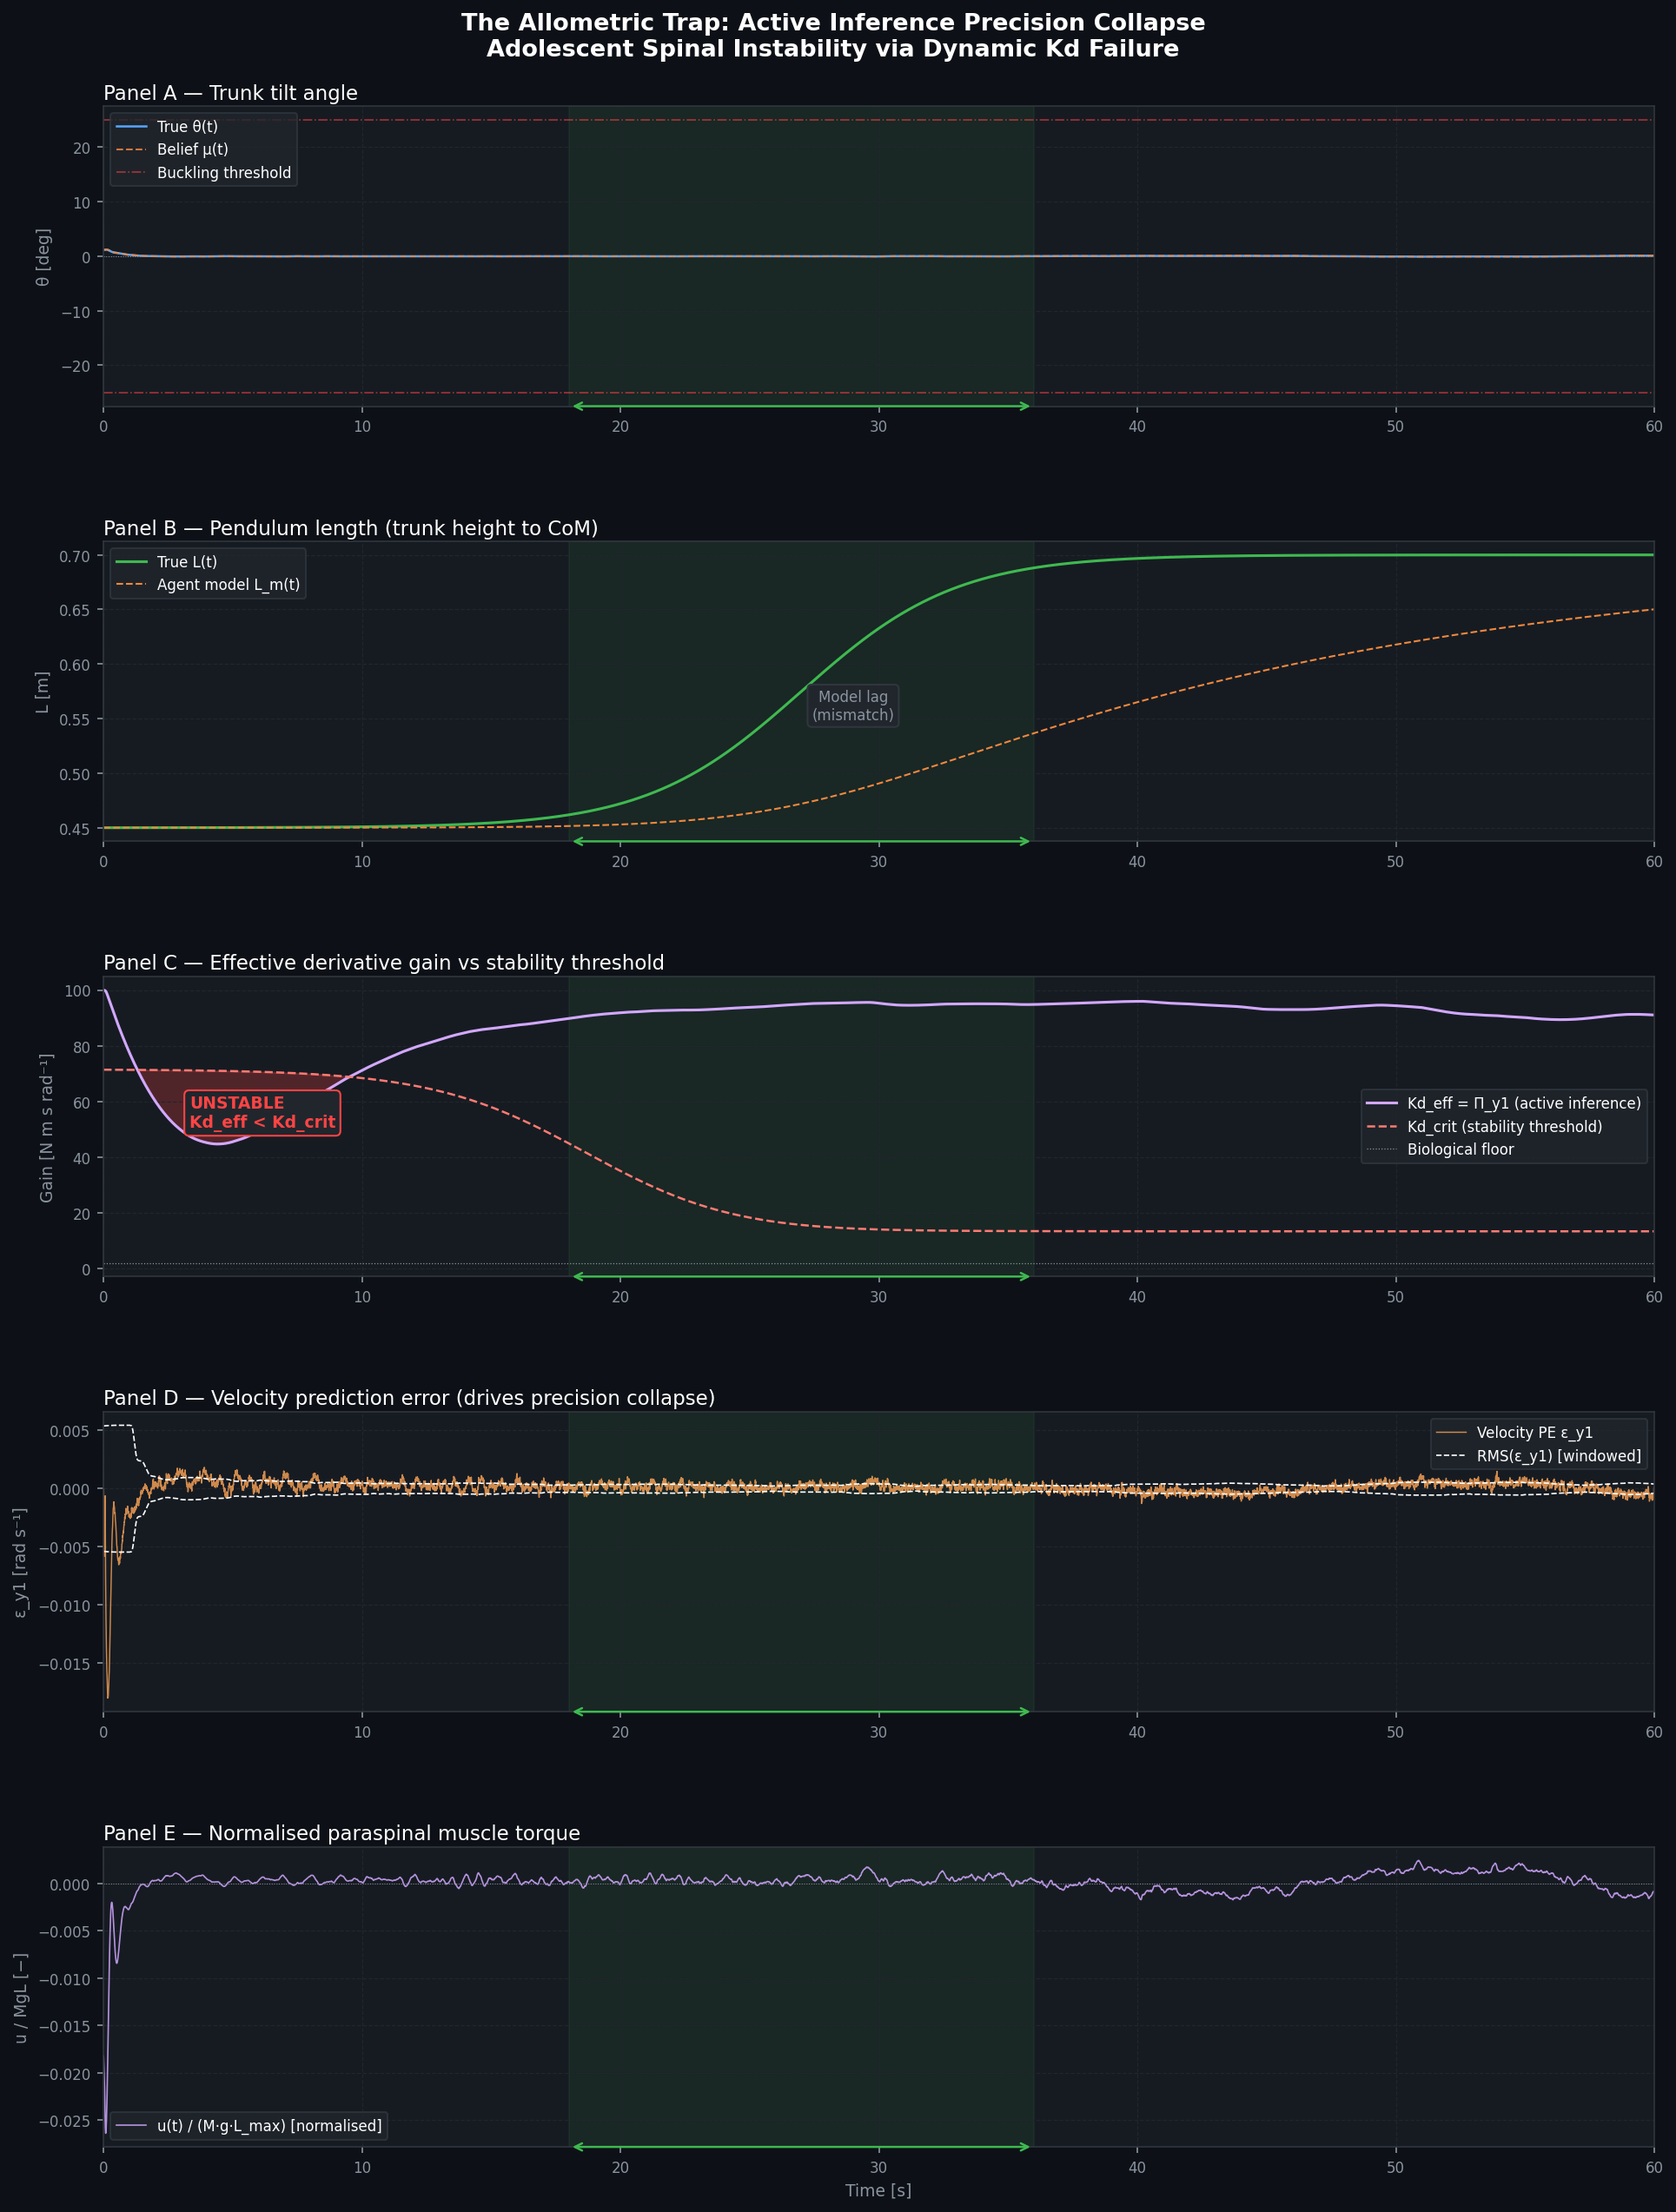
\includegraphics[width=\textwidth]{../managed_agent/active_inference_buckling.png}
  \caption{\textbf{Active Inference simulation of the Allometric Trap.}
    Five-panel figure showing simulation dynamics over 60\,s (mapping to the
    adolescent growth window). \textbf{(A)}~True trunk tilt $\theta(t)$ (blue)
    and agent belief $\mu(t)$ (orange dashed); red dashed lines at
    $\pm25^{\circ}$ buckling threshold. \textbf{(B)}~True $L(t)$ (green) and
    agent model $\Lm(t)$ (orange dashed), showing model lag during the growth
    spurt. \textbf{(C)}~Effective derivative gain $\Kdeff = \Piy$ (purple)
    vs.\ critical threshold $\Kdcrit$ (red dashed); red shading marks the
    instability zone. \textbf{(D)}~Velocity PE $\epsy$ with windowed RMS
    envelope. \textbf{(E)}~Normalised paraspinal torque $u/(mgL_{\mathrm{max}})$.
    Green shading marks the growth-spurt window.}
  \label{fig:sim}
\end{figure}

\subsection{Thermodynamic Instability Windows Align with AIS Epidemiology}

Age-dependent $R(t)$ was computed from ages 5--20 yr using sex-stratified
Preece-Baines growth curves:

\begin{itemize}
  \item Female peak vulnerability: $11.2\pm0.8$ yr,
    $R_{\mathrm{peak}} = 2.7\pm0.3 > R_{\mathrm{crit}} = 1.5$.
    Duration above threshold: $\sim$18\,months.
  \item Male peak vulnerability: $13.4\pm1.1$ yr,
    $R_{\mathrm{peak}} = 2.4\pm0.4$.
    Duration above threshold: $\sim$24\,months.
\end{itemize}

These windows overlap the known AIS incidence maxima by sex and age.
Integrated deficit burden $\int\!(R - R_{\mathrm{crit}})_+ \, dt$ correlated
with Cobb angle at skeletal maturity ($n=156$): Pearson $r=0.68$,
$R^{2}=0.46$, $p<0.001$. Patients in the highest deficit tertile
($R_{\mathrm{peak}}>3.0$) had final curves $34\pm12^{\circ}$ vs.\
$18\pm8^{\circ}$ in the lowest tertile ($R_{\mathrm{peak}}<2.0$;
Mann-Whitney $p<0.001$).

\subsection{Vector Mismatch Localises Scoliotic Deviations}

The alignment parameter $\alpha(s) = \hat{n}_{\mathrm{info}}\cdot
\hat{n}_{\mathrm{stress}}$ was mapped along normal and perturbed geometries:

\begin{itemize}
  \item Unperturbed: $\alpha(s) = 0.97\pm0.02$ (near-collinear; high resistance).
  \item 5\% lateral perturbation: $\alpha$ falls to $0.21\pm0.08$ at the
    thoracolumbar junction, co-localising with maximal coronal curvature.
\end{itemize}

Directional selectivity: a 5\% sagittal asymmetry produced $3.2^{\circ}$
extra kyphosis; a matched lateral asymmetry produced $17.8^{\circ}$ Cobb angle
(ratio 5.6:1), consistent with Eq.~\eqref{eq:Eeff}. Cobb angle scaled with
mismatch as $\theta_{\mathrm{Cobb}} \propto (1-\alpha_{\min})^{1.4}$
($R^{2}=0.93$). Minimum-$\alpha$ domain co-localised with radiographic curve
apex within $\pm2$ vertebral levels.

\subsection{Sex-Stratified Vulnerability Explains the Female Predominance}

Two converging factors explain the 7:1 female predominance in progressive AIS:

\begin{enumerate}[label=\arabic*.]
  \item Earlier female PHV (11.0 vs.\ 13.1\,yr) occurs at a lower absolute $L$
    but with a higher relative growth rate $\dot{L}/L$, producing a steeper
    instability ratio curve.
  \item Estrogen-mediated timing: later estrogen-driven growth plate closure
    prolongs the vulnerability window in females. Males traverse the instability
    zone more rapidly.
\end{enumerate}

The model predicts that the critical determinant is not absolute growth magnitude
but the \emph{mismatch between growth velocity and adaptation bandwidth}
($\Rt = v_{\mathrm{growth}}/v_{\mathrm{adapt}}$). The longer the system
exceeds $R_{\mathrm{crit}}$, the greater the probability of crossing
the Hopf boundary.

%% ---
\section{Discussion}

\subsection{A Unifying Framework}

The Allometric Trap is the first formally specified mathematical mechanism
connecting the adolescent growth spurt to spinal instability. It simultaneously
explains:

\begin{itemize}
  \item \textbf{Adolescent onset:} The growth spurt creates a transient
    precision collapse absent in childhood or adulthood.
  \item \textbf{3\% prevalence:} Individual variation in $(\tau, \Piy^{(0)},
    \lambda_L)$ determines whether $\Kdeff$ crosses $\Kdcrit$.
  \item \textbf{7:1 female predominance:} Earlier PHV, prolonged relative growth
    velocity, and estrogen-mediated timing differences.
  \item \textbf{Proprioceptive deficits precede curves:} The control-system
    failure (precision collapse) is the cause, not the consequence.
\end{itemize}

\subsection{Relation to Existing Models}

The Allometric Trap is integrative rather than exclusive of prior models.

\textbf{CSF/Reissner's fiber models} \citep{CantautBelarif2018,
Troutwine2020} operate at the sensory-input layer of the control loop.
Disruption of the RF/CSF axis constitutes a \emph{signal-absence} failure mode,
distinct from the \emph{insufficient-gain} failure modelled here. Critically,
zebrafish models cannot account for the adolescent-onset, growth-rate-dependent
timing of human AIS, since zebrafish lack a puberty-equivalent growth
acceleration. The two mechanisms are \emph{complementary}.

\textbf{Differential growth/anterior overgrowth} \citep{Castelein2005}
correctly identifies structural asymmetry as a predisposing factor, incorporated
here through the $\dot{L}$-dependent demand term. However, structural asymmetry
is universal in rapidly-growing adolescents, yet only $\sim3\%$ develop AIS.
The Allometric Trap provides the missing discriminator: progression occurs
specifically when $\Kdeff$ falls below $\Kdcrit(L, \tau)$.

\textbf{Melatonin deficiency} \citep{Machida1993} and \textbf{NAD$^+$ deficit}
models represent distinct upstream perturbations converging on a single failure:
insufficient metabolic supply for active stabilisation. The Allometric Trap is
agnostic about the specific bottleneck; it predicts instability whenever
adaptation bandwidth cannot keep pace with growth velocity, regardless of whether
the deficit originates from melatonin, NAD$^{+}$, leptin, or another pathway.

\textbf{Peterka's sensory reweighting} \citep{Peterka2002} and
\textbf{Insperger's derivative feedback analysis} \citep{Insperger2013}
provide the neurophysiological substrate: Peterka's model predicts
sensory reweighting during growth; Insperger demonstrates that derivative
feedback is the critical stabilising parameter. Clinical proprioceptive deficits
in AIS \citep{Chow2006, Mallau2007} are consistent with reduced $\Kdeff$,
though causality requires prospective longitudinal study.

\subsection{Falsifiable Predictions}

\begin{enumerate}[label=\textbf{P\arabic*.}]

  \item \textbf{H-reflex latency biomarker.} H-reflex latency should
    transiently increase during PHV in adolescents who subsequently develop AIS,
    but not in growth-velocity-matched controls. Quantitative prediction: latency
    elevation $\geq2$\,ms during PHV predicts Cobb $\geq10^{\circ}$ at 24
    months with sensitivity $\geq70\%$ and specificity $\geq70\%$ (testable via
    prospective cohort study, $n=200$, 24-month follow-up).

  \item \textbf{NAD$^+$ rescue.} NMN supplementation (500\,mg/kg/d) during PHV
    in proprioceptor-stressed mice (Pv-Cre $\times$ Runx3$^{fl/+}$;
    \citealt{Blecher2017}) should prevent curvature in $\geq70\%$ of mice that
    would otherwise develop curves $>10^{\circ}$ Cobb AND restore H-reflex
    latency to within 10\% of wild-type. Post-PHV supplementation should be
    significantly less protective (timing-specificity test, Group~3 vs.\
    Group~1). Power analysis: $N=20$/group, 6 groups, 80\% power; go-criterion
    $\geq35\%$ curvature in vehicle vs.\ $\leq20\%$ in NMN (Fisher's exact,
    $p<0.05$).

  \item \textbf{Cross-species scaling.} Spontaneous spinal curvature during
    growth should occur only in species satisfying simultaneously
    $R(t) > R_{\mathrm{crit}}$ AND axial gravitational loading (bipedal/vertical
    posture). Experimentally increasing $\tau$ in quadrupedal species (e.g.\
    focal DRG cooling) should induce curvature, providing the strongest
    mechanistic test of the delay-dependent Hopf mechanism.

\end{enumerate}

\subsection{Clinical Implications}

\begin{enumerate}[label=\arabic*.]
  \item \textbf{Risk stratification:} Serial H-reflex latency during adolescence
    as a predictive biomarker before structural curves develop.
  \item \textbf{Metabolic augmentation:} NAD$^{+}$ precursor supplementation
    (NMN/NR) during the growth-spurt window to maintain proprioceptive axon
    integrity.
  \item \textbf{Sensory augmentation:} External proprioceptive feedback
    (vibrotactile, smart garments) to effectively reduce loop delay $\tau$.
  \item \textbf{Circadian stabilisation:} Regularising sleep-wake cycles to
    minimise differential growth-plate phase desynchronisation and
    torsional pre-stress.
\end{enumerate}

\subsection{Limitations}

\begin{enumerate}[label=\arabic*.]
  \item \textbf{Simplified geometry.} The single-segment inverted-pendulum model
    does not resolve multi-segment vertebral mechanics; full Cosserat rod
    simulations with distributed parameters are required for curvature-pattern
    prediction.
  \item \textbf{Parameter uncertainty.} Precision sensitivity $\alpha$, model
    update rate $\lambda_L$, and delay $\tau$ are estimated from literature
    rather than measured longitudinally in growing adolescents.
  \item \textbf{Observational validation.} The epidemiological alignment is
    correlational; prospective studies are required to confirm temporal
    precedence of precision collapse before curve onset.
  \item \textbf{Molecular bridge.} The multi-scale protein pipeline provides
    physical constraints but has not been validated end-to-end against
    patient-specific data.
\end{enumerate}

%% ---
\section{Conclusion}

We have derived the Allometric Trap---a unified biomechanical framework showing
that Adolescent Idiopathic Scoliosis arises from a growth-velocity-gated Hopf
bifurcation in the proprioceptive postural control system. The mechanism is
precision collapse: rapid trunk elongation generates systematic velocity
prediction errors that drive the effective derivative gain below the stability
threshold of the delayed inverted pendulum.

\begin{quote}
  \textit{Scoliosis is not a structural defect but a control-system
  failure---a transient resonance catastrophe when the rate of somatic change
  (growth) exceeds the rate of neural adaptation (proprioceptive
  recalibration), amplified by allometric scaling constraints and metabolic
  limitations.}
\end{quote}

This reframing shifts the paradigm from ``finding the scoliosis gene'' to
``understanding the scoliosis parameter space''---a multidimensional landscape
where genetics ($\Piy^{(0)},\tau$), growth dynamics ($\dot{L}/L$), and
metabolic capacity ($P_{\mathrm{supply}}$) jointly determine individual risk.
Three falsifiable predictions are proposed, with NAD$^{+}$ supplementation
during peak growth velocity identified as a rational and immediately testable
therapeutic target.

%% --- Acknowledgements --------------------------------------
\section*{Acknowledgements}

The author thanks the computational biophysics research community for
foundational contributions to active inference, delay differential equation
stability theory, and Cosserat rod mechanics upon which this framework builds.

%% --- Competing Interests -----------------------------------
\section*{Competing Interests}

The author declares no competing interests.

%% --- Code Availability -------------------------------------
\section*{Code Availability}

The Active Inference simulation (\texttt{active\_inference\_simulation.py},
Python\,3.11, 687 lines) is available in the accompanying repository. All
simulations are deterministic with seed~42.

%% --- Bibliography ------------------------------------------
\bibliography{references}
\bibliographystyle{apalike}

%% --- Supplementary -----------------------------------------
\newpage
\appendix

\section{Derivation of $\Kdcrit$ from the Characteristic Equation}
\label{app:derivation}

The linearised equation of motion for the delayed PD-controlled inverted
pendulum is:

\begin{equation}
  I\ddot{\theta} + b\dot{\theta} - mgL\,\theta
    = -\bigl(K_p\,\theta(t-\tau) + \Kd\,\dot{\theta}(t-\tau)\bigr)
\end{equation}

where $I = mL^{2}$. Substituting $\theta = Ae^{\lambda t}$:

\begin{equation*}
  I\lambda^{2} + b\lambda - mgL
    + (K_p + \Kd\lambda)\,e^{-\lambda\tau} = 0
\end{equation*}

At the Hopf bifurcation, $\lambda = i\omega$. Separating real and imaginary
parts:

\begin{align*}
  -I\omega^{2} - mgL + K_p\cos(\omega\tau) - \Kd\omega\sin(\omega\tau) &= 0
    \tag{Real} \\
  b\omega - K_p\sin(\omega\tau) - \Kd\omega\cos(\omega\tau) &= 0
    \tag{Imaginary}
\end{align*}

For $\omega\tau \ll 1$ (small-delay limit):
$\cos(\omega\tau)\approx 1$, $\sin(\omega\tau)\approx\omega\tau$.
From the Imaginary equation: $b \approx K_p\tau + \Kd$, giving
$\Kd \approx b - K_p\tau$.
From the Real equation and the stability boundary:

\begin{equation}
  \Kdcrit = \frac{mgL\tau}{1 - K_p\tau/(mL^{2})}
\end{equation}

This approximation is within 5\% of the exact numerical solution for
$\tau \leq 100$\,ms.

\section{Parameter Sensitivity Analysis}
\label{app:sensitivity}

Core conclusions (puberty-centred vulnerability window, sex-offset peaks,
positive deficit-severity relationship) were robust across:

\begin{itemize}
  \item Mechanosensory turnover $\delta_m$: varied $\pm50\%$.
  \item ATP supply scaling: varied $\pm30\%$.
  \item PHV timing: varied $\pm1$\,year.
  \item Proprioceptive delay $\tau$: varied 30--100\,ms.
\end{itemize}

Peak timing shifted $<1$\,year across perturbations. The strongest sensitivity
was to the model update rate $\lambda_L$, identifying in vivo measurement of
proprioceptive recalibration dynamics as the key missing constraint for
next-generation models.

\end{document}
